\documentclass[openany]{scrbook}

\KOMAoptions{parskip=half}


\usepackage[utf8]{inputenc}
\usepackage[ngerman]{babel}
\usepackage[T1]{fontenc}
\usepackage{xcolor}
\usepackage{graphicx}
\usepackage[german=guillemets]{csquotes}
\usepackage[breaklinks=true]{hyperref}
\usepackage[clearempty]{titlesec}
\usepackage{a4wide}


\title{Bachelorarbeit-Mini}
\subtitle{Tetrahydrocannabinol}
\author{Angelique Siebert 645834}
\date{11.12.2016}

\begin{document}
	\maketitle
	\tableofcontents

	\chapter
	{Tetrahydrocannabinol}
	\section{Einleitung}
	\textbf{Tetrahydrocannabinol} (THC) zählt zu den psychoaktiven Cannabinoiden und ist der hauptsächlich rauschbewirkende Bestandteil der Hanfpflanze (Cannabis). Tetrahydrocannabinol unterliegt in Deutschland den Bestimmungen des Betäubungsmittelgesetzes.
	
\begin{figure}[h]
	\centering
	
\includegraphics[width=6cm]{C:/Users/Franz/Desktop/abb1}
	\caption{Strukturformel von THC}
	\label{fig:THC}
\end{figure}

\section{Chemie}
	Tetrahydrocannabinol wurde in reiner Form erstmals 1964 von Yehiel Gaoni und Raphael Mechoulam am Weizmann-Institut für Wissenschaften in Israel isoliert.\footnote[1]{ Yehiel Gaoni, Raphael Mechoulam: Isolation, structure and partial synthesis of an active constituent of hashish. In: Journal of the American Society. 86, Nr. 8, 1964, S. 1646–1647, doi:10.1021/ja01062a046} Gewonnen wird THC hauptsächlich aus der Hanfpflanze (Cannabis). Besonders reich an THC sind hierbei die unbefruchteten weiblichen Blütenstände (etwa 6 bis 20\%),der THC-Gehalt der übrigen Pflanzenteile ist weit geringer (knapp 1\%). In den Samen der Pflanze ist gar kein THC enthalten. Die Blätter nahe der Blüte enthalten etwa 5–6 \% THC. Männliche Pflanzen haben im Unterschied zu weiblichen einen sehr geringen THC-Gehalt. 
	
\begin{figure}[h]
	\centering
	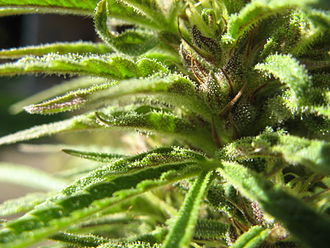
\includegraphics[width=4cm]{C:/Users/Franz/Desktop/abb2}
	\caption{Weibliche Blütenstände}
	\label{fig:Fe}
\end{figure}

\subsection{Biosythese}
	Tetrahydrocannabinol liegt in der Cannabis-Pflanze überwiegend als THC-Säure vor. Durch enzymatische Kondensation aus den beiden Prekursoren Geranylpyrophosphat und Olivetolsäure wird Cannabigerolsäure gebildet, die anschließend enzymatisch in Tetrahydrocannabinolsäure umgelagert wird. Durch Wärme und UV-Strahlung decarboxyliert die Säure zum THC. Eine Umwandlung oral aufgenommener THC-Carbonsäure in THC ließ sich in Fütterungsexperimenten mit Ratten nicht nachweisen.\footnote[2]{J. Jung, M. R. Meyer, H. H. Maurer, C. Neusüß, W. Weinmann, V. Auwärter: Studies on the metabolism of the Delta9-tetrahydrocannabinol precursor Delta9-tetrahydrocannabinolic acid A (Delta9-THCA-A) in rat using LC-MS/MS, LC-QTOF MS and GC-MS techniques. In: Journal of Mass Spectrometry. 44, Nr. 10, 2009, S. 1423–1433, doi:10.1002/jms.1624}
	
\begin{figure}[h]
	\centering
	
\includegraphics[width=4cm]{C:/Users/Franz/Desktop/abb3}
	\caption{Biosythese von THC-COOH}
	\label{fig:800px-THC_biosynthesis}
\end{figure}

\subsection{Extraktion}
	THC ist sehr lipophil. Es kann per Extraktion aus THC-haltigem Pflanzenmaterial isoliert werden, wozu unpolare und schwach polare Lösungsmittel wie n-Alkane, Aceton, Isopropylalkohol oder Ethanol geeignet sind. Nach dem Abdampfen des Lösungsmittels bleibt ein harziger, ölartiger Extrakt zurück. Die Zusammensetzung des Extrakts ist abhängig von der Wahl des Lösungsmittels. Bei geeigneten Bedingungen können sehr hohe THC-Konzentrationen erreicht werden. Dieser Extrakt wird auch als Haschischöl bezeichnet.
	
	Mit n-Butan lassen sich lipophile Inhaltsstoffe bei sehr tiefen Temperaturen aus dem Pflanzenmaterial extrahieren; diese Methode bringt allerdings hohe Brand- und Explosionsgefahr mit sich. Butan verdampft bereits bei Zimmertemperatur. Der so erhaltene Extrakt hat ein Aussehen ähnlich wie Bernstein, bei Zimmertemperatur ist er dickflüssig und zieht Fäden wie Kunstharz. Wenn man ihn abkühlt, erstarrt er relativ schnell.
	
	Neben THC enthält der Extrakt weitere Cannabinoide; bei Verwendung stärker polarer Extraktionsmittel wie Ethanol können entsprechend polare Stoffe enthalten sein, wie Chlorophyll, Alkaloide (Trigonellin, Hordenin), Aminosäuren, Aminozucker,\footnote[3]{ Eberhard Breitmeier: Alkaloide. Teubner, Stuttgart 1997, ISBN 3-519-03542-1, S. 87 ff.} eventuell auch ungelöste feine Teile des Ausgangsmaterials. Durch geeignete Verfahren kann der Extrakt noch weiter gereinigt werden.
	
\begin{figure}[h]
	\centering
	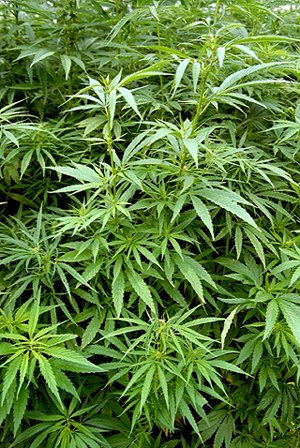
\includegraphics[width=6cm]{C:/Users/Franz/Desktop/abb4}
	\caption{Hanf (Cannabis sativa) enthält – je nach Sorte – wechselnde Mengen (–)-$\Delta^9$-trans-Tetrahydrocannabinol (THC).}
	\label{fig:Cannabis_sativa}
	\end{figure}
	
\subsection{Teilsynthese}
		\textbf{Dronabinol} ist teil-synthetisch produziertes Tetrahydrocannabinol. In Deutschland wird es von den Unternehmen Bionorica Ethics und THC Pharm produziert. Dronabinol-haltige Fertigarzneimittel sind bisher in Deutschland nicht zugelassen. In den Vereinigten Staaten sowie Kanada gibt es unter dem Handelsnamen Marinol Fertigarzneimittel in Kapselform, die gemäß § 73 Abs. 3 AMG importiert werden können. Meistens wird jedoch Dronabinol als Rezeptursubstanz für Dronabinol-Kapseln oder ölige Dronabinol-Tropfen verschrieben.\footnote[4]{http://www.pharmazeutische-zeitung.de/fileadmin/nrf/PDF/1-Dronabinol.pdf} Ein synthetisches Analogon ist Benzopyranoperidin (Nabitan, Nabutam).
		
		Der Wirkstoff wird aus rechtlichen Gründen mit aufwendigen Verfahren aus THC-armem Nutzhanf teilsynthetisch hergestellt (Extraktion von Cannabidiol und Umwandlung in THC) und ist daher sehr viel teurer, als wenn man ihn aus potentem „Rauschhanf“ extrahieren würde.
		
		Die Wirkungsweise und die Indikation entsprechen denen von Tetrahydrocannabinol (siehe korrespondierende Abschnitte unten).
		
\subsection{Konsumformen von Cannabis}
	Sofern THC durch Cannabis-Konsum aufgenommen wird, ist die häufigste Konsumform das Rauchen von Haschisch oder Marihuana pur oder gemischt mit Tabak als Joint. Häufig wird THC-haltiges Material auch mit Hilfe speziellen Rauchzubehörs wie Bongs und Pfeifen geraucht oder mit dem Vaporizer verdampft und inhaliert.
	
	Daneben wird THC auch in Speisen und Getränken verarbeitet. Da THC lipophil ist, kann es in fettreichen Nahrungsmitteln wie Milch, Kuchen, Muffins verarbeitet werden. THC ist auf Grund seiner Lipophilie ohne Emulgator nicht intravenös applizierbar. Aufgrund seiner schlechten Wasserlöslichkeit kann es in Form von Lösungen oder Emulsionen mit Ethanol, Dimethylsulfoxid, Polysorbat 80, Cremophor EL oder Polyvinylpyrrolidon verabreicht werden.
	
\section{Pharmakologie}	
\subsection{Wirkmechanismen}

\begin{figure}[h]
	\centering
	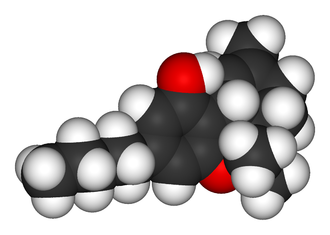
\includegraphics[width=6cm]{C:/Users/Franz/Desktop/abb5}
	\caption{Kalottenmodell des Tetrahydrocannabinols}
	\label{fig:800px-Tetrahydrocannabinol-3D-vdW}
\end{figure}

		Der Wirkmechanismus von THC ist nicht vollständig geklärt.
		
		THC wirkt auf mindestens zwei Arten von Rezeptoren, die bei Säugetieren vorkommen, $CB_1$ und $CB_2$. $CB_1$-Rezeptoren befinden sich vorwiegend in zentralen und peripheren Nervenzellen, wo sie die Ausschüttung von Neurotransmittern modulieren. Sie kommen aber auch in anderen Zellen vor, zum Beispiel in der Hypophyse, Immunzellen, gastrointestinalem Gewebe, sympathetischen Ganglien, Herz, Lunge, Harnblase und Nebennieren. $CB_2$-Rezeptoren kommen hauptsächlich in Immunzellen vor und sind an der Zytokinausschüttung beteiligt.
		
		Endocannabinoide sind körpereigene Substanzen, die auf die $CB_1$- und CB2-Rezeptoren wirken. Sie sind Eikosanoide und werden vom Organismus bei Bedarf erzeugt. Die bekanntesten sind Arachidonylethanolamid (Anandamid) und 2-Arachidonylglycerol (2-AG). Die Endocannabinoide und die Cannabinoid-Rezeptoren bilden das sogenannte Endocannabinoid-System.
		
		THC bindet an die $CB_1$-Rezeptoren und beeinflusst die Signalübertragung an diesen Synapsen, mit Auswirkungen auf das zentrale und periphere Nervensystem, wie Glücksgefühl, Entspannung und Analgesie (Schmerzlinderung). Die Aktivierung hemmt über G-Proteine die Adenylylcyclase, blockiert Ca2+-Kanäle und aktiviert K+-Kanäle. Die Transduktionsmechanismen ähneln hierbei den Opioidrezeptor-Subtypen $\mu,\sigma$ und $\kappa.$
		
		Über die Rolle der CB2-Rezeptoren ist weniger bekannt, man nimmt jedoch an, dass sie an der Immunmodulation beteiligt sind, weil sie vorwiegend in B-Zellen und in natürlichen Killerzellen vorkommen.
		
		Im Tiermodell wirkt THC antagonistisch auf 5-HT3-Rezeptoren, welche am Brechreiz beteiligt sind.
		
		THC wirkt auch auf andere pharmakologische Ziele, wie auf Capsaicin empfindliche perivaskuläre sensorische Nerven.
		
		Das Verteilungsmuster der CB1-Rezeptoren im Gehirn bedingt viele der pharmakologischen Eigenschaften von THC. Im Stammhirn, wo lebenswichtige Funktionen wie Atmung koordiniert werden, sind nur sehr wenige bis gar keine dieser Rezeptoren vorhanden. Im Hippocampus, wo das Kurzzeitgedächtnis angesiedelt ist, finden sich hingegen viele dieser Rezeptoren. CB1-Rezeptoren in den Basalganglien bieten eine Erklärung für den Einfluss von THC auf die Motorik.
		
		Das schwach psychoaktive Cannabidiol (CBD) hat neben eigenen therapeutischen Wirkungen einen modulierenden Einfluss auf THC. Sowohl THC als auch CBD wirken antioxidativ und entfalten so eine neuroprotektive Wirkung, zum Beispiel bei Glutamat-induzierter Excitotoxizität. THC hemmt die Glutamat-Ausschüttung, möglicherweise auch den Eintritt von Calcium über die Ionenkanäle, und könnte deshalb eine neuroprotektive Wirkung entfalten.
		
		Das in Cannabis in geringer Menge enthaltene $\Delta^8$-Tetrahydrocannabinol ($\Delta^8$-THC) ist psychoaktiv, aber etwas weniger potent als $\Delta^9$-THC.
		
		THC und CBD können Zeichen des apoptotischen und nekrotischen Zelltods bei Tumorzellen induzieren.
		

\subsection{Toxizität}
	Die LD50 bei der Maus beträgt 42 mg/kg Körpergewicht intravenös und 482 mg/kg bei oraler Verabreichung, beim Rhesusaffen tritt nach intravenöser Gabe von 128 mg/kg Körpergewicht der Tod durch Atemstillstand und Herzversagen ein.\footnote[7]{Eberhard Teuscher, Ulrike Lindequist: Biogene Gifte. Akademie-Verlag, Berlin 1988, Letale Dosen von THC bei Maus und Rhesusaffe, S. 65 f.}
	
	Der LD50-Wert wird am Menschen nicht ermittelt und lässt sich nicht verlässlich hochrechnen. Nimmt man in einer groben (und niedrig angesetzten) Schätzung, den potentiellen peroralen LD50-Wert für Menschen mit 150 mg/kg Körpergewicht an, dann würde eine 70 kg schwere Person nach oralem Akut-Konsum von 10,5 g THC mit einer Wahrscheinlichkeit von 50 \% sterben. Diese Menge ist enthalten in rund 70–130 g eines Cannabisprodukts mit 8 – 15 \% THC-Gehalt. Andere Autoren geben niedrigere letale Dosen von etwas über 4 Gramm an.\footnote[5]{ Lester Grinspoon, James B. Bakalar: Marihuana, die verbotene Medizin. Zweitausendeins, Frankfurt am Main 1994, ISBN 3-86150-060-4.} Da THC über den Darm nur zu etwa 6 \% und über die Lunge zu rund 20 \% resorbiert wird, ist es praktisch unmöglich, letale Mengen THC durch den Konsum natürlicher Cannabisprodukte zuzuführen, zumal die erforderliche Menge um etwa den Faktor 1000 über der üblichen Konsummenge liegt. Es ist beim Menschen kein Fall einer Überdosis mit Todesfolge durch Aufnahme natürlicher Cannabisprodukte bekannt;\footnote[8]{J. Michael Walker, Susan M. Huang: Cannabinoid analgesia. In: Pharmacology \& Therapeutics. 95, Nr. 2, 2002, S. 127–35. doi:10.1016/S0163-7258(02)00252-8. „…to date, there are no deaths known to have resulted from overdose of cannabis. (S. 128)“} das synthetische THC-Produkt „Marinol“ (auch „Dronabinol“) war hingegen in den USA nach Aussage der FDA für 4 von 11.687 Todesfällen durch insgesamt 17 verschiedene FDA approved drugs zwischen dem 1. Januar 1997 und dem 30. Juni 2005 verantwortlich.\footnote[9]{Deaths from Marijuana v. 17 FDA-Approved Drugs (PDF; 121 kB) 30. Juni 2005. Abgerufen am 3. Februar 2011.}	
	
	
\subsection{Pharmakokinetik}
	Psychische Effekte treten bei folgenden Dosierungen auf: 30–50 microg/kg intravenös, 50 microg/kg bei Rauchinhalation, 120 microg/kg oral.Bei Rauchinhalation geringerer Mengen THC (5–7 mg) überwiegt die sedative Komponente, bei Mengen von 15 mg oder darüber überwiegt Vigilanz, die sich bis zu psychotischen Zuständen steigern kann.
	
	Bei Rauchinhalation gehen ungefähr 20 \% des im Rauch vorhandenen $\Delta^9$-THC in das Blut über, oral nur etwa 6 \%. THC geht vom Rauch sehr schnell ins Blut über, hierbei ist die Entwicklung der Plasmakonzentration mit intravenöser Einnahme vergleichbar. Bei oraler Einnahme in Form von Sesamölkapseln ist die Wirkung wegen des First-Pass-Effekts vermindert, die Bioverfügbarkeit beträgt nur etwa 10 bis 20 \%, die höchste THC-Konzentration wird nach etwa zwei Stunden erreicht.
	
	THC ist im Blutplasma überwiegend an Proteine gebunden; maximal 10 \% kommen in den roten Blutkörperchen vor. Die Plasmahalbwertszeit nach intravenöser Gabe entwickelt sich in vier Phasen, was nahelegt, dass es mindestens vier Gewebearten gibt, in die THC einsickert, mit jeweils unterschiedlicher Durchlässigkeit und Bindungskapazität. Nach starker Verringerung in den ersten Minuten sinkt die THC-Konzentration nur noch langsam. Die Halbwertszeiten der ersten drei Phasen betragen jeweils 1 Minute, 4 Minuten und 1 Stunde. Die anfänglich kurze Halbwertszeit ist auf den schnellen Übergang von THC in bestimmte Gewebearten sowie auf die schnelle Verstoffwechslung der Substanz zurückzuführen. Nach ungefähr 6 Stunden besteht ein Pseudogleichgewicht zwischen dem THC-Gehalt im Blutplasma und in den Geweben. Die Halbwertszeit der vierten Phase (terminale Halbwertszeit nach Erreichen des Pseudogleichgewichts) wird unterschiedlich mit 19–36 Stunden angegeben. Nach 5 Tagen ist etwa 80 bis 90 \% des THC in Form von Metaboliten ausgeschieden, etwa zu zwei Dritteln im Stuhl und zu einem Fünftel im Harn.
	
	Die THC-Konzentration im Gehirn erreicht nach rund 30 Minuten ihr Maximum; die Konzentration ist drei- bis sechsmal höher als im Plasma. Die THC-Konzentrationskurven im Gehirn und im Plasma verlaufen parallel, was für ein uneingeschränktes Passieren der Blut-Hirn-Schranke spricht. Tierversuche haben gezeigt, dass sich THC als lipophile Substanz in bestimmten Gewebearten stark anreichert, zum Beispiel in Körperfett, Herz, Leber und Lunge. Ebenso wurde im Tierversuch nachgewiesen, dass THC durch die Plazenta auf Föten übergeht. Welche Auswirkungen dies hat, ist weitgehend unbekannt.
	
\subsection{Syntehtische Analoga}
	 \begin{tabular}[pos]{l|lr}
	 	\textbf{Wirkstoff}&\textbf{Wirkung}\\ \hline
	 	$\Delta$6a,10a-THC & eventuell psychoaktiv \\
	 	$\Delta$6a,10a-Dimethylheptyl-THC & DMH-THC, teilweise psychoaktiv\\
	 	Nabilon & Antiemitikum, psychoaktiv \\
	 	CP-47,497 & Analgetikum, psychoaktiv
	 \end{tabular}
	 
\subsection{Wirkungen}
	Bekannte Wirkungen von $\Delta^9$-THC auf den Menschen beziehungsweise Wirkungen von Cannabis, die auf $\Delta^9$-THCzurückgeführt werden: \\
	
	\begin{tabular}{p{5cm}|p{5cm}|p{5cm}}
		\textbf{Effekte mit therapeutischen Potenzial} & \textbf{Effekte des high} & \textbf{Andere Wirkungen} \\ \hline
		\begin{itemize}
			\item Analgesie, Linderung neuropathischer und entzündungsbedingter Schmerzen
			\item Wirkung auf motorische Funktionen, Linderung von Spastizität
			\item Neuroprotektion
			\item Hemmung der gastrointestinalen Motilität
			\item Antiemetische Wirkung (Linderung von Übelkeit und Erbrechen)
			\item Senkung des Augeninnendrucks
			\item Erleichterung des Schlafes
			\item Appetitanregende Wirkung
			\item Hemmende Wirkung auf die Ausbreitung von Krebszellen
		\end{itemize}
		& 
		\begin{itemize}
			\item Stimmungssteigerung
			\item Euphorie
			\item Redseligkeit
			\item Veränderte Wahrnehmung (z. B. in Bezug auf Farben, Musik, Geschmack und Zeitgefühl)
			\item Gefühle erhöhter Einsicht und Bedeutung
		\end{itemize}
		&
		\begin{itemize}
			\item Beeinträchtigung des Denk-, Lern- und Erinnerungsvermögens
			\item Beeinträchtigung des Konzentrationsvermögens
			\item Beeinträchtigung der psychomotorischen Leistung, Ataxie, Tremor
			\item Gefühle von Unwirklichkeit, Depersonalisation und Distanzierthei
			\item Unterbrechung von Gedankengängen
			\item Panik, Angst, Dysphorie
			\item Begünstigt psychotische Symptome, Paranoia
			\item Auswirkungen auf kardiovaskuläre Funktionen, einschließlich Tachykardie und Haltungshypotonie
			\item Bindehautrötung, verminderter Tränenfluss, Mundtrockenheit
			\item Wirkungen auf endokrine und reproduktive Funktionen
			\item Wirkungen auf die Thermoregulation
			\item Mydriasis
		\end{itemize}
	
		
	\end{tabular} \\
	
	Bei regelmäßigem, intensivem Konsum kann sich ein Toleranzeffekt (erforderliche Dosissteigerung, um die gewohnte Wirkung zu erzielen) entwickeln. Entzugssymptome und eine damit einhergehende Entwicklung von Abhängigkeit sind bedingt durch eine Unterfunktion des mesolimbischen Systems (subkortikale Belohnungssysteme), die nach Absetzen des Konsums wirksam wird und andauert bis sich in diesen Arealen ein neuronales Gleichgewicht (Entwöhnung) wieder hergestellt hat.
	
	Eine Vielzahl von Studien hat zu der heute unstrittigen Erkenntnis geführt, dass Cannabiskonsum mit einem erhöhten Risiko für die Auslösung psychotischer Erkrankungen verbunden ist. Ferner steigt das Risiko mit der Menge des Konsums. Ein ursächlicher Zusammenhang ist bislang jedoch noch nicht gefunden worden. Deshalb bleibt unklar, ob Cannabis hier als alleiniger Faktor oder nur in Kombination mit anderen als Auslöser auftritt. Als möglicher neurobiologischer Mechanismus wurde eine durch Cannabinoide verursachte Störung dopaminerger Systeme diskutiert.
	
	Wird Cannabis geraucht, entstehen bei seiner Verbrennung ähnlich wie beim Tabak krebserregende Produkte. Wird es als Joint, also als Mischung mit Tabak geraucht, kommen die Risiken des Nikotinkonsums, wie z. B. das Risiko einer Arteriosklerose, hinzu.
	
	Es bestehen keine Hinweise, dass THC selbst mutagen, karzinogen oder teratogen (fruchtschädigend) ist. Schwangere und Stillende sowie Heranwachsende sollten auf den Konsum von THC verzichten, weil Schäden am ungeborenen oder gestillten Kind nicht ausgeschlossen werden können und es Hinweise darauf gibt, dass THC die Entwicklung des nicht ausgereiften Gehirns nachhaltig beeinflussen könnte. Dazu liegen auch zahlreiche Erkenntnisse aus tierexperimentellen Studien vor.
	
	Metaanalysen von 2013 und 2014, die die bis dahin vorliegenden Gehirnstudien durch bildgebende Verfahren auswerteten, gelangten zu dem Ergebnis, dass Cannabiskonsum im präfrontalen Cortex (Stirnseite des Frontallappens der Großhirnrinde) zu einem verminderten Gehirnvolumen und zu einer Beeinträchtigung der weißen Substanz (Nervenverbindungen) führt, sowie zu einem beidseitigen verminderten Volumen des Hippocampus. Bei letzterer Gehirnregion, die eine Schlüsselrolle bei allen Gedächtnisfunktionen hat, bestand zusätzlich eine Korrelation (Entsprechung) zwischen Volumenabnahme und Menge des bisherigen Cannabiskonsums.
	
	

	
	
\end{document}